\chapter{Investigating the Subgroup Diagnosis} \label{ch:meas}
\thispagestyle{plainbottom}
The dataset collected in different labs consists of different groups of diagnosis. Each of these diagnosis is dependent on the features of the reviews. In this chapter, analysis of these groups has been done using different Machine Learning techniques. For the purpose of understanding the diagnosis, initially unsupervised learning technique (k-means clustering) is applied. Then, feature selection algorithms are applied to understand the feature importance of our entire data available. Finally, supervised learning techniques have been applied to predict each of these different groups diagnosis. Also, the features of the data are divided into four sections (IQ, ADI, BASC, VINE) and supervised learning techniques have been applied to predict the diagnostic label using each section of features.

\section{Unsupervised Learning Techniques to Categorize Subjects}
The dataset is clustered using $K$-Means Clustering algorithm to analyze the clusters in the dataset. The dataset consists of 73 features/variables after the preprocessing of our data. For applying $K$-Means clustering, the dimension of the data has to be reduced further and for this purpose Principal Component Analysis\nomenclature{PCA}{Principal Component Analysis} has been used. The PCA transforms the set of features of the dataset orthogonally. Also, PCA handles the missing values and the outliers in our data, so for this section of our analysis missing values have not be handled as part of preprocessing. For the given dataset, the PCA algorithm in sklearn package in python is used. For visualizing our dataset, the PCA algorithm is applied to find the first two principle components of our dataset, so that our data can be visualized in 2D. After performing PCA, the figure \ref{fig:41} gives the visualization of our dataset. From this figure, it can be seen that there are four different/unique groups. However, there is an overlap between 2 groups as children diagnosed with `ASD+ADHD` and falling into the group of children diagnosed with `ASD`. Similarly, children diagnosed with `VCFS+ASD` fall into the group of children diagnosed with `VCFS`. Due to this overlap there are only two distinguishable majority groups in our subgroup data.
\begin{figure}
\centering
  {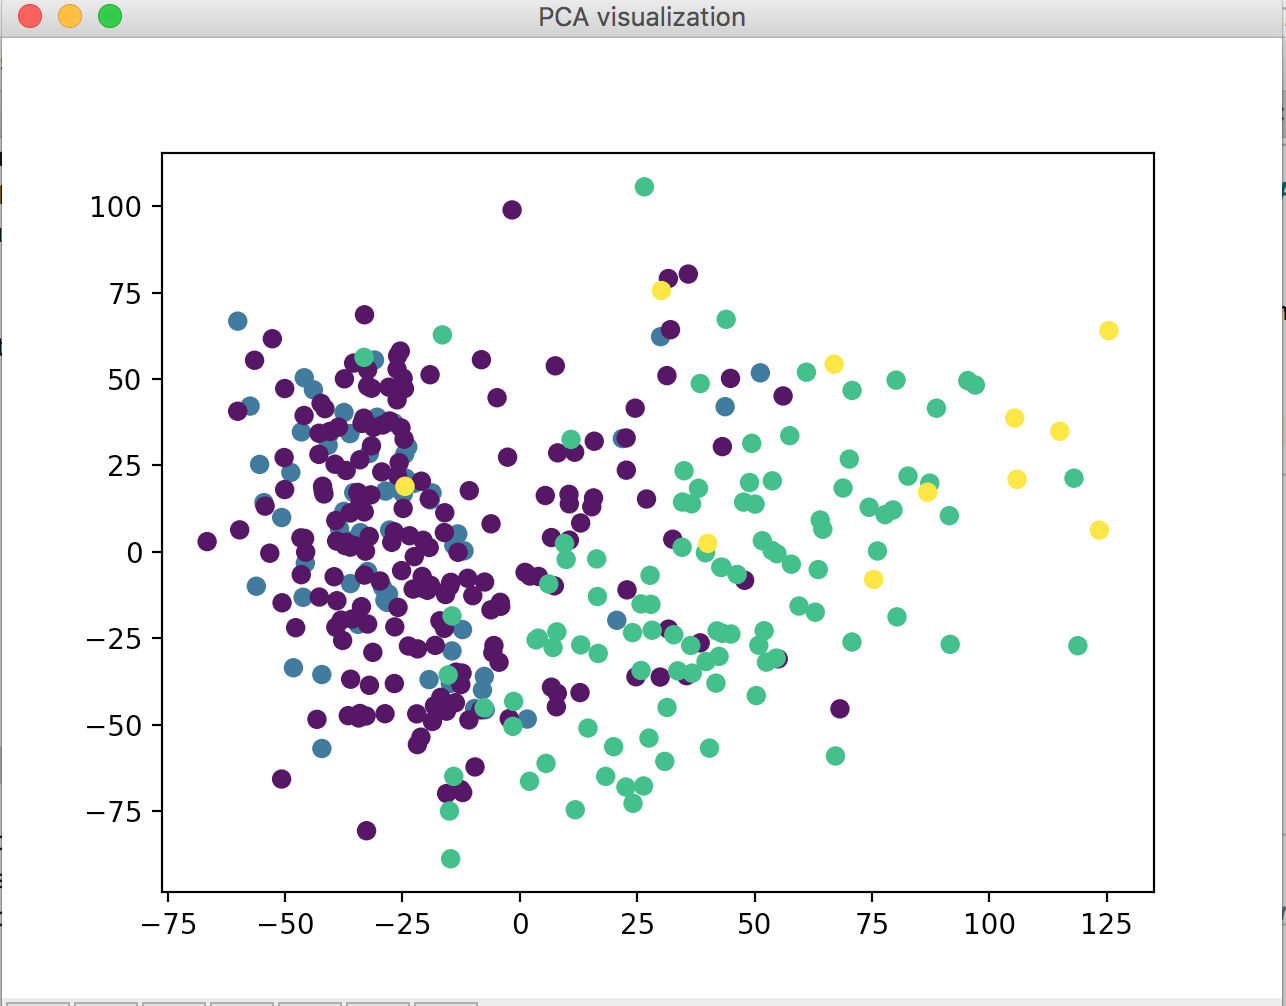
\includegraphics[width=0.6\textwidth]{Figures/Figure_4_1.png}}
  \caption{Analyzing missing values of features in BASC}
  \label{fig:41}
\end{figure}
Now, on this reduced data from PCA has been given as input to K-Means clustering algorithm without the diagnostic labels. The $K$-Means clustering algorithm available in sklearn package has been used. As proper analysis of the data needs to be done, the $k$ value was varied from 2 to 5. Since, there are 4 different diagnostic groups in our dataset, the data has been cluster unto $k$ value equal to 5. The main reason behind this is to check if there are any pure clusters. For each of these $k$ values, the visualization is given in the figure \ref{fig:42}.

In the figure \ref{fig:42}, when $k$ is equal to 2, cluster 1 (yellow color) consists of  all VCFS diagnosed children (including children with VCFS+ASD) and cluster 2(purple color) has ASD and ASD+ADHD diagnostic children. However, there are 16 children in cluster 1 who have ASD only and 1 child in cluster 1 having ASD+ADHD. Then, the cluster size was increased to 3 and it was observed that cluster 1 consisted of all the VCFS+ASD children. Further analysis showed that children with ASD and ASD+ADHD were spread over all the three clusters, whereas children with VCFS only were spread over first two clusters. When the cluster size was increased further to 4 and 5, it was observed that the clusters where more of a mixture, there was no purity in the clusters. The main reason for this could be that there are lot of features overlap for each of the diagnostics.
\begin{figure}
\centering
  {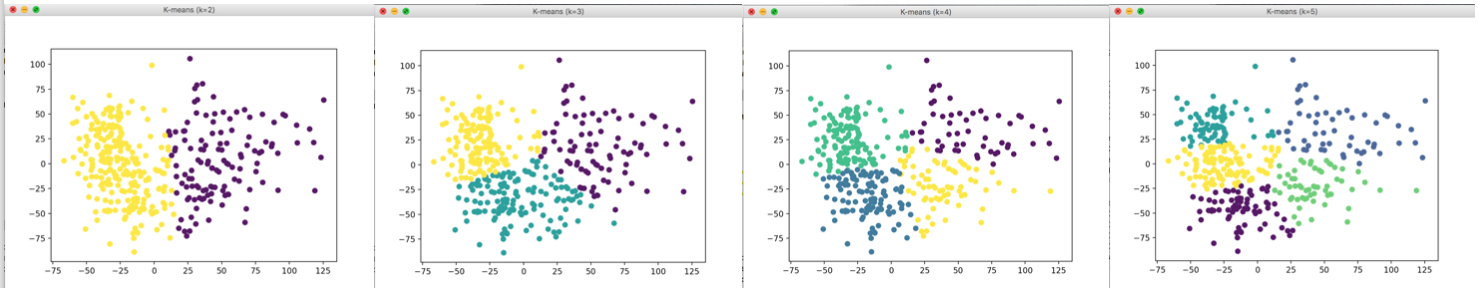
\includegraphics[width=0.9\textwidth]{Figures/Figure_4_2.png}}
  \caption{After applying $k$-means clustering on the PCA reduced dataset}
  \label{fig:42}
\end{figure}
% * <reza@data.syr.edu> 2018-04-12T18:02:07.357Z:
%
% ^.

As mentioned above, PCA handles missing values, if the preprocessed data were given as input to the K-Means then the accuracy of the K-Means clustering algorithm dropped to 83.5\%, that means that there was more randomness in the data and higher chances of not grouping them accurately. However, the average accuracy of clustering the data was 95.3\%. After, K-means clustering it could be said that children diagnosed with VCFS are closely clustered that is they belonged to one cluster most of the times and more specifically children with VCFS+ASD were most likely to be in the same cluster than the other diagnostic subgroups.

\section{Supervised Learning Techniques to Predict Diagnostic Groups}
The subgroup dataset after preprocessing is trained using different supervised learning techniques. As the dataset is small and simple, there is no need for very complex classification models. The data is loaded into WEKA and different classification algorithms have been applied on this data. The algorithms are compared based on different metrics as seen in table \ref{table:41}. The different metrics on which the models are evaluated are Accuracy, Precision, Recall, ROC Area and F-measure. Cross validation technique has been applied on the data and the dataset has been divided into 10 folds wherein training is done on 9 folds and testing on one. The different classification algorithms that have been used to train our models are Naive Bayes, Logistic Regression, Multi-class classifier and Random Forest. Since, our dataset consists of feature relations and multiple class labels, the above algorithms were chosen.
%table 4.1
\begin{table}[h]
\begin{center}
\begin{tabular}{|l|c|c|c|c|c|}
\hline
\textbf{ML Algorithm} & \textbf{Precision}&	\textbf{Recall}&	\textbf{F-measure}&	\textbf{ROC Area}&	\textbf{Accuracy}\\
\hline \hline
Naive Bayes & 0.934 &	0.924 &	0.928 &	0.981& 	92.4119\%\\
\hline
Logistic Regression &	0.926&	0.924&	0.924&	0.990&	92.4119\%\\
\hline
Multi Class Classifier&	0.902&	0.902&	0.902&	0.980&	90.2439\%\\
\hline
Random Forest&	0.960	&0.959	&0.957	&0.994&	94.85\%\\
\hline
\end{tabular}
\end{center}
\caption{Supervised learning techniques to predict subgroup diagnosis}
\label{table:41}
\end{table}

Among the different supervised learning techniques applied on the dataset, Random Forest has a better accuracy and ROC Area value.\nomenclature{ROC}{Receiver Operator Characteristic} So, it can be said that Random Forest is doing a good job of classifying our dataset. Also, each of the class labels are measured to check their precision and recall. For the group of children diagnosed with ASD+ADHD, precision and recall of Random Forest is 96.6\% and 90.5\% respectively. Similarly the precision and recall for the children diagnosed with ASD is 93.9\% and 96.3\% respectively. For the children diagnosed with VCFS, precision and recall are 95.4\% and 100\% respectively. However, precision and recall for the children with VCFS+ASD is 100\% and 45\% respectively and this could be because their are a low percentage of children with VCFS+ASD when compared to the other diagnostic groups.   Now, rather than giving the entire feature set, only the best features selected from the three different feature selection algorithms as in chapter 3 are given to machine learning algorithms to predict our subgroup diagnosis. The results of each of the feature selection algorithms are given below in table \ref{table:42} by LASSO and table \ref{table:43} by RFE.
%table 4.2
\begin{table}[h]
\begin{center}
\begin{tabular}{|l|c|c|c|c|}
\hline
\textbf{ML Algorithm} & \textbf{Accuracy}&	\textbf{Precision}&	\textbf{Recall}&	\textbf{ROC Area}\\
\hline \hline
Naive Bayes&	66\%	&0.690&	0.656&	0.851\\
\hline
Logistic Regression&	73\%&	0.605&	0.732&	0.827\\
\hline
Multi Class Classifier&	72.6\%	&0.584	&0.7267&	0.829\%\\
\hline
Random Forest&	70.4\%&	0.680&	0.705	&0.859\%\\
\hline
\end{tabular}
\end{center}
\caption{Supervised learning techniques to predict subgroup diagnosis by LASSO}
\label{table:42}
\end{table}

%table 4.3
\begin{table}[h]
\begin{center}
\begin{tabular}{|l|c|c|c|c|}
\hline
\textbf{ML Algorithm} & \textbf{Accuracy}&	\textbf{Precision}&	\textbf{Recall}&	\textbf{ROC Area}\\
\hline \hline
Naive Bayes&	83.1\%	&0.836&	0.832&	0.924\\
\hline
Logistic Regression&84.2\%&	0.842&	0.843&	0.917\\
\hline
Multi Class Classifier&	84.2\%&	0.841&	0.843&	0.916\\
\hline
Random Forest&84.5\%&	0.840&	0.846&	0.912\\
\hline
\end{tabular}
\end{center}
\caption{Supervised learning techniques to predict subgroup diagnosis by RFE }
\label{table:43}
\end{table}
From the tables \ref{table:42} and \ref{table:43}, the features selected from the RFE feature selection are preforming better than out LASSO feature selection algorithm. However, when using only the best 5 features, the accuracy of the random forest drops from 96\% to 84\% but the ROC Area value is still high in the case of Random forest. Also, with the help of LASSO features we selected all the relevant features with non-zero weights. Out of the 73 features after preprocessing, the relevant features were 45 and when Random forest model was trained on these 45 features, an accuracy of 92\% was achieved. 
\begin{figure}
\centering
{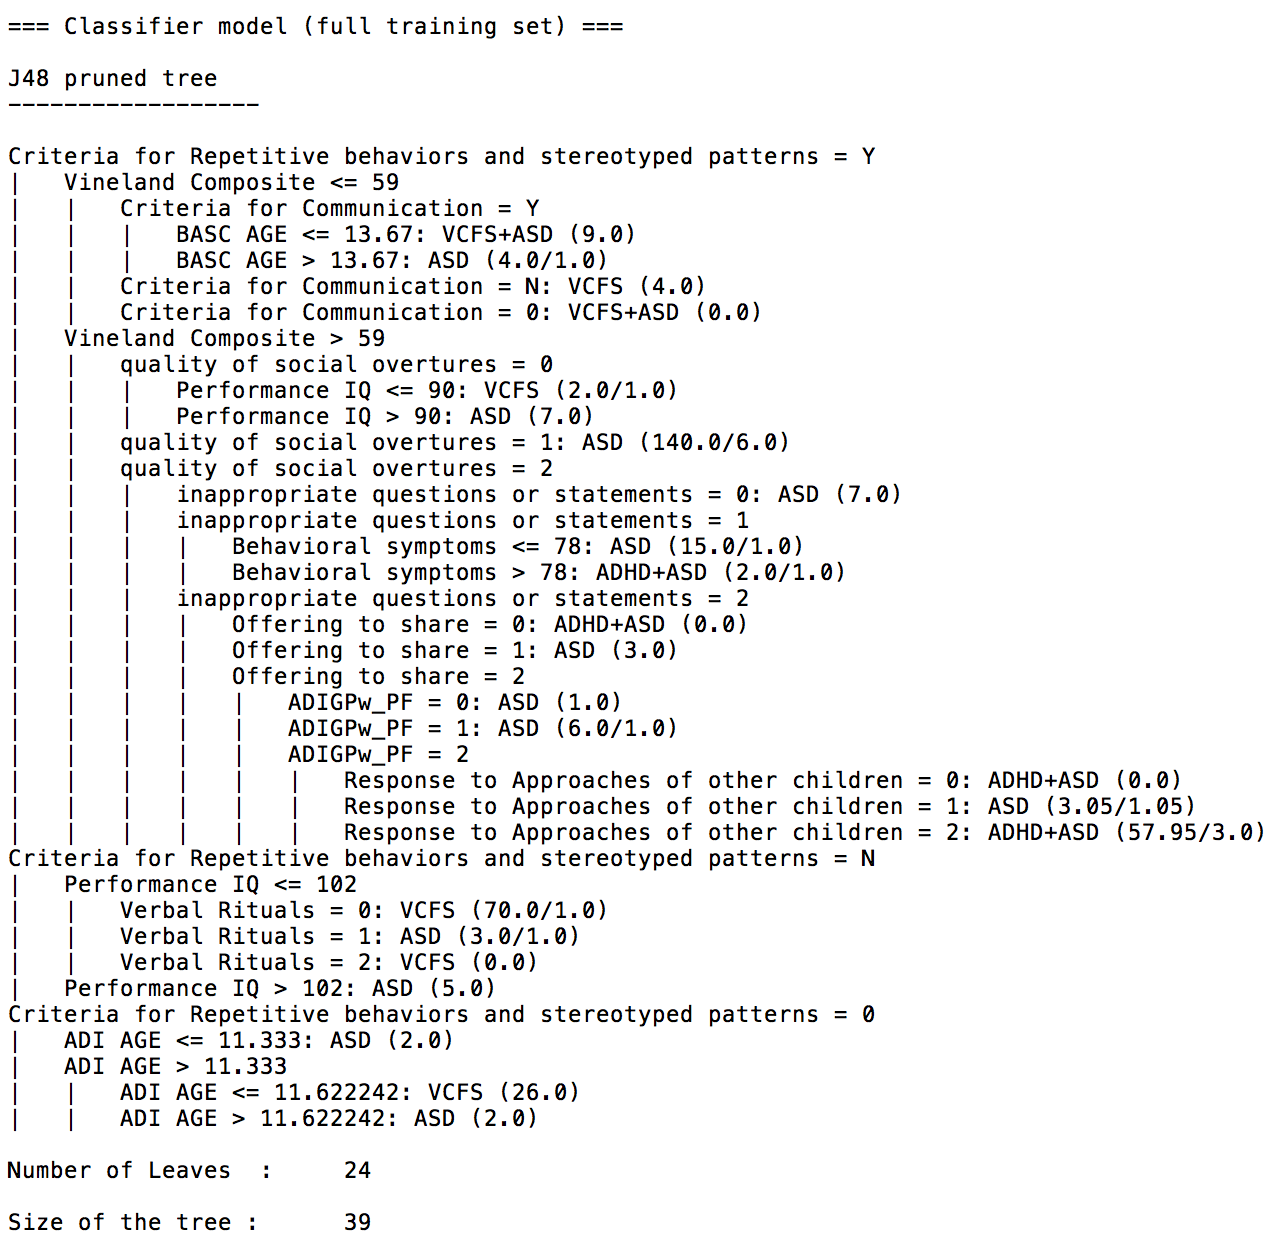
\includegraphics[width=0.5\textwidth]{Figures/Figure_4_3.png}}
  \caption{J48 pruned tree}
  \label{fig:43}
\end{figure}

Since, Random Forest is doing a good job at predicting the subgroup features, another types of tree algorithm J48 also known as ID3 from WEKA is used to represent our model in the form of the tree. The figure \ref{fig:43} shows the results obtained from the J48 algorithm.It had an accuracy, precision and recall of 87\%. Also, precision and recall for the subgroups ASD, ASD+ADHD, VCFS ranges from 81\% to 90\%, however, the precision and recall for VCFS+ASD group is 60\%.

\subsection{Predicting Subgroup Diagnosis using the IQ feature set}
In this section of our research, IQ feature set consists of 3 features and using only these features, the subgroup diagnosis of the data is predicted. So, only these 3 features are given to our machine learning algorithms and the results are observed in table \ref{table:44}.
%table 4.4
\begin{table}[h]
\begin{center}
\begin{tabular}{|l|c|c|c|c|c|}
\hline
\textbf{ML Algorithm} &	\textbf{Precision}&	\textbf{Recall}&	\textbf{F-measure}& \textbf{ ROC Area}&	\textbf{Accuracy}\\
\hline \hline
Random Forest&	0.604&	0.623&	0.612&	0.802&	66.32\%\\
\hline
Naive Bayes&	0.401&	0.485&	0.438&	0.612&	48.50\%\\
\hline
Logistic Regression&	0.546&	0.580&	0.517&	0.716&	57.99\%\\
\hline
\end{tabular}
\end{center}
\caption{Supervised learning techniques to predict subgroup diagnosis by IQ feature set}
\label{table:44}
\end{table}

When all the different machine learning algorithms are compared, then Random forest is performing better than other machine learning algorithms. However, the Random forest has very low accuracy of 66\%. It has dropped from 92\% to 66\% which is very low and not an accurate model for the purpose of prediction. In this case, it could be mainly because the IQ range is similar for all the diagnostic groups.

\subsection{Predicting Diagnosis based on ADI feature set}
The ADI review has 45 features/variables in the dataset that analyze the behavior of children. These attributes are used to predict the diagnosis of the child. Initially, many supervised techniques have been applied on the Subgroup data and the various metrics of evaluation are listed in the table \ref{table:45}. 
%table 4.5
\begin{table}[h]
\begin{center}
\begin{tabular}{|l|c|c|c|c|c|}
\hline 
\textbf{Classifier} &	\textbf{Precision} &	\textbf{Recall} &	\textbf{F-measure} & \textbf{ROC Area}&	\textbf{Accuracy}\\
\hline \hline
Random Forest	&0.966&	0.965&	0.964&	0.976&	96.47\%\\
\hline
Naive Bayes&0.876	&0.870&	0.869&	0.959&	86.99\%\\
\hline
Logistic Regression&0.868&	0.864	&0.866&	0.936&	86.44\%\\
\hline
\end{tabular}
\end{center}
\caption{Supervised learning techniques to predict subgroup diagnosis by ADI feature set}
\label{table:45}
\end{table}

When using the reduced feature set from LASSO, which consisted of 45 features, these features were a combination of all the three parent-oriented reviews and the accuracy of our Random Forest model was 92\%. However, when we use only the 45 ADI features , the accuracy of our Random Forest model is 96\% with high precision and recall. Since, random forest model is doing great when predicting the subgroup diagnosis with ADI feature set, another similar algorithm J48 has been applied to our data. this will help our model to be concisely visualized in the form of a tree. The results of J48 in the form of a tree are given in figure \ref{fig:44}. The accuracy of our model is 87\%.

\begin{figure}
\centering
  {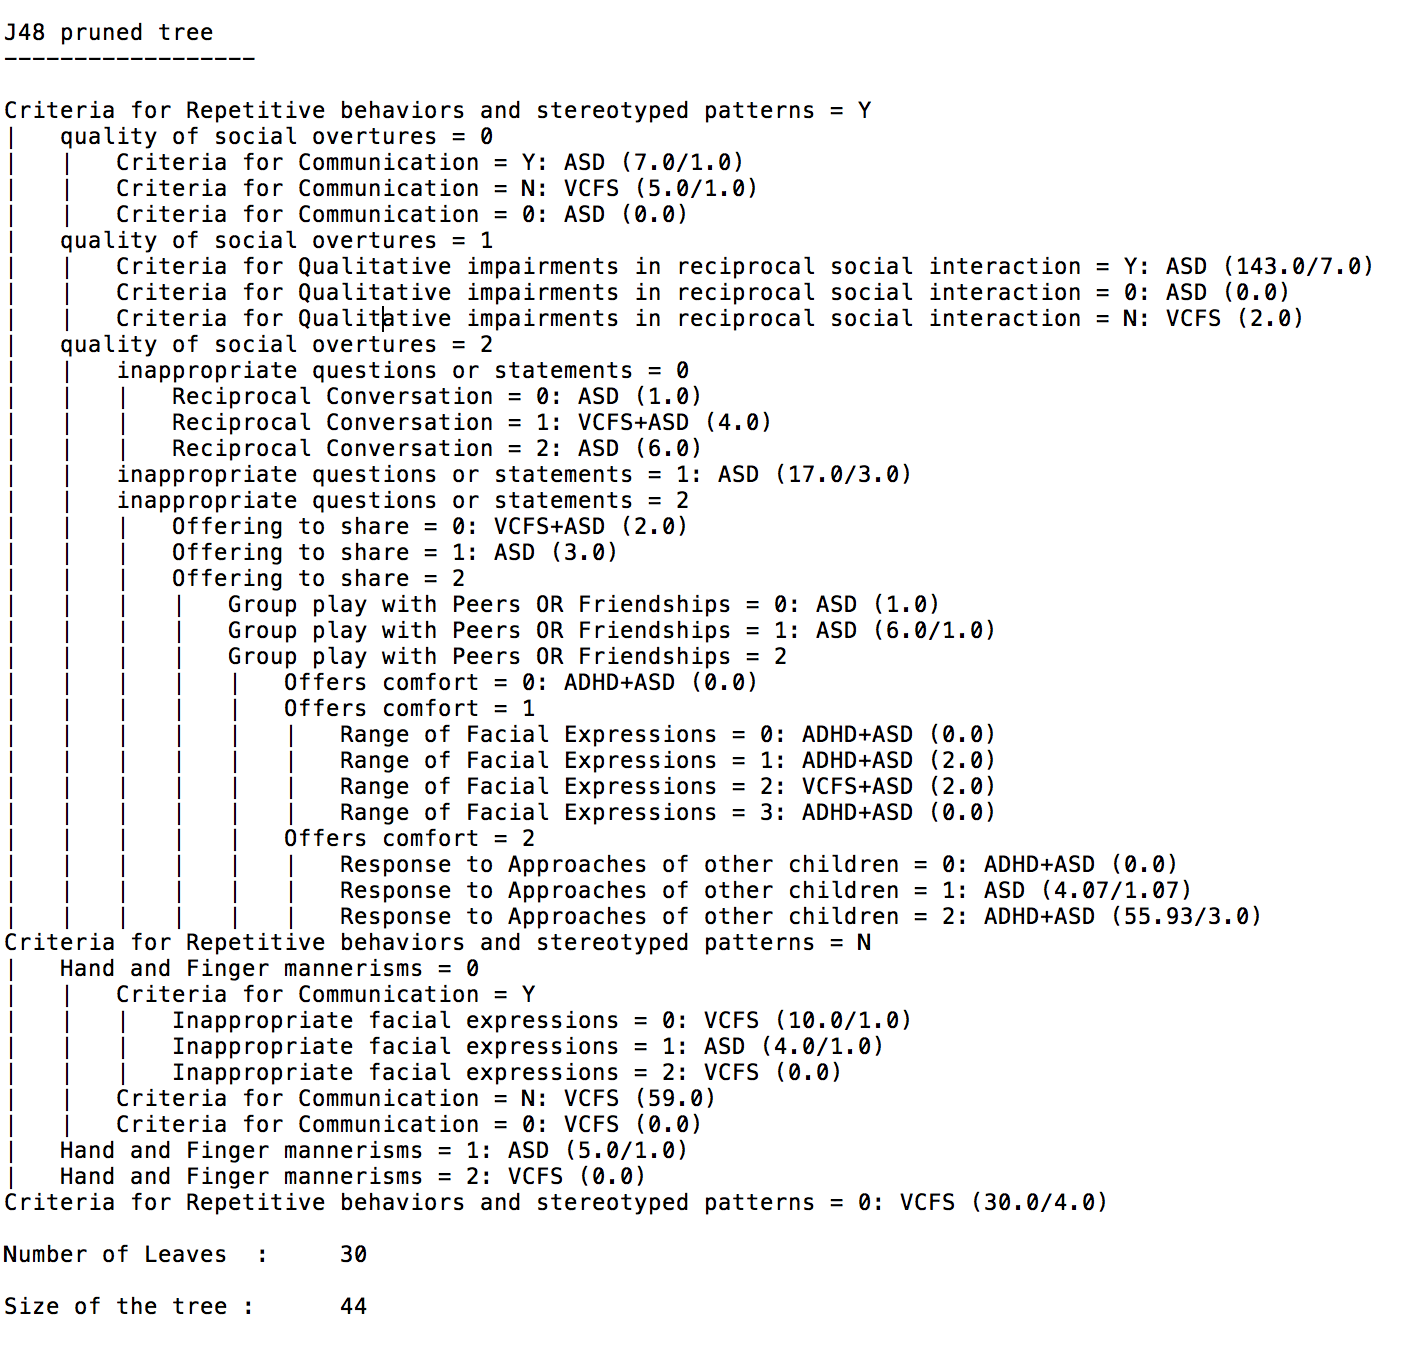
\includegraphics[width=0.6\textwidth]{Figures/Figure_4_4.png}}
  \caption{J48 pruned tree with ADI feature set}
  \label{fig:44}
\end{figure}

\subsection{Predicting Diagnosis based on BASC feature set}
BASC is another parent-oriented review where there are 19 different features to analyze the behaviors of the children. These features of BASC are used to predict the diagnosis of the child. Initially, many supervised techniques have been applied on the Subgroup data diagnosis and the various metrics of evaluation are listed in the table \ref{table:46}. 
%table 4.6
\begin{table}[h]
\begin{center}
\begin{tabular}{|l|c|c|c|c|c|}
\hline
\textbf{ML Algorithm} &	\textbf{Precision}&	\textbf{Recall}&	\textbf{F-measure}& \textbf{ROC Area}&	\textbf{Accuracy}\\
\hline \hline
Random Forest&0.713	&0.751&	0.712	&0.879&	75.06\%\\
\hline
Naive Bayes&0.694	&0.659&	0.671	&0.841&	65.85\%\\
\hline
Logistic Regression&0.693	&0.713	&0.694&	0.861&	71.27\%\\
\hline
\end{tabular}
\end{center}
\caption{Supervised learning techniques for subgroup diagnosis by BASC feature set}
\label{table:46}
\end{table}

Random Forest is performing better than all other machine learning algorithms with an accuracy of 75.06\%, but this accuracy is not high for predicting subgroup diagnosis as compared to previous models of predictions.

\subsection{Predicting Diagnosis based on VINE feature set}
VINE is also another parent questionnaire, when compared to other two reviews, VINE has fewer features for analyzing the behaviors. Also, the children who have taken the VINE tests are less compared to other two tests. These 4 features of VINE are used to predict the diagnosis of the child. Initially, many supervised techniques have been applied on the Subgroup data and the various metrics of evaluation are listed in the table \ref{table:47}. In the case of VINE parent-oriented review, the best model is by Logistic Regression with an accuracy of 71\% and the random forest only gives an accuracy of 68\%. 
%table 4.7
\begin{table}[h]
\begin{center}
\begin{tabular}{|l|c|c|c|c|c|}
\hline
\textbf{ML Algorithm} &	\textbf{Precision}&	\textbf{Recall}&	\textbf{F-measure}& \textbf{ROC Area}&	\textbf{Accuracy}\\
\hline \hline
Random Forest& 0.560&	0.680&	0.612&	0.785&	68.02\%\\
\hline
Naive Bayes& 0.550&	0.553&	0.517&	0.600&	55.28\%\\
\hline
Logistic Regression& 0.656&	0.710&	0.680&	0.787&	71\%\\
\hline
\end{tabular}
\end{center}
\caption{Supervised learning techniques for subgroup diagnosis by VINE feature set}
\label{table:47}
\end{table}

\section{Observations}
The machine learning algorithms applied to distinguish the subgroups are doing good job and the results are great. Among all the machine learning algorithms that have been applied on our actual data, Random Forest is doing well at predicting our subgroup diagnosis labels. This shows that  the model is successfully at finding the required relations between the feature set to the diagnostic labels. Using LASSO feature selection algorithm, the features were reduced from 72 to 45 and the performance of the Random Forest model is still very good. This shows that not all the 72 features are required to predict the diagnosis of the children with different combinations of these developmental disorders.

Apart from this when the feature set was divide into four different sub features set, it was observed that using the IQ features, the BASC parent-oriented review features and VINE parent-oriented review features can not be used individually to define models that can predict the subgroup diagnosis accurately. On the other hand, ADI parent-oriented reviews have resulted in good models when predicting the subgroup diagnosis features. The Random Forest model designed with ADI features is better than the Random Forest model built with 45 features from LASSO. Also, the J48 pruned tree with the entire feature set has similar model performance as the J48 pruned tree with only ADI parent-oriented reviews, that is both models have an accuracy of 87\%. When the ADI features are analyzed in more depth, it could be seen that some of the important features as selected by the J48 algorithm among the 45 ADI features are as follows:
\begin{compactenum}
\item Criteria for Repetitive behaviors and stereotyped patterns
\item Criteria for Qualitative impairments in reciprocal social interaction
\item Inappropriate questions and statements
\item Offers Comfort
\item Quality of social overtures
\item Offering Comfort
\item Range of Facial Expressions 
\item Hand and finger mannerisms
\item Response to approaches of other children
\item Reciprocal Conversation
\end{compactenum}

Most of the features that have been selected are key symptoms of the developmental diagnosis that our research is trying to predict in the children. This shows that our models are able to find valuable information like this from our features. As models built with ADI features are doing well and comparable with the entire feature set, it can be said that ADI features are sufficient. Therefore, ADI parent-oriented review is better than BASC and VINE parent-oriented review for building models to predict the subgroup diagnosis.